\section{结构化观测}
\label{sec:observation}

本节呈现$5 \times 3$实验矩阵的实证观测。我们建立三个关键发现：(1) 分支级性能结构确实存在且显著；(2) logit蒸馏相比定位蒸馏并非最优；(3) 分支排序在轻度-中度条件下呈现部分稳定性，但在重度退化下出现显著例外。

\subsection{核心性能矩阵}

\Cref{tab:core_matrix}呈现所有KD分支和可见度等级的完整性能矩阵。若干模式立即可见。

\begin{table}[htbp]
\centering
\caption{核心性能矩阵（mAP@50），跨KD分支和可见度等级。每列最佳结果加粗。}
\label{tab:core_matrix}
\begin{tabular}{@{}lccc@{}}
\toprule
KD分支 & 轻度（$\beta=0.005$） & 中度（$\beta=0.01$） & 重度（$\beta=0.02$） \\
\midrule
仅学生（基线） & 0.5828 & 0.5873 & 0.5625 \\
仅logit & 0.5866 & 0.5811 & 0.5678 \\
仅特征 & 0.5861 & 0.5874 & 0.5576 \\
仅注意力 & 0.5853 & 0.5776 & \textbf{0.5721} \\
\textbf{仅定位} & \textbf{0.5952} & \textbf{0.5906} & 0.5606 \\
\bottomrule
\end{tabular}
\end{table}

\textbf{发现1：分支级结构存在。}性能在分支间不均匀。定位蒸馏在轻度和中度可见度下达到最高mAP@50（分别为0.5952和0.5906），而注意力蒸馏在重度下表现最佳（0.5721）。这证明不同KD机制对可见度退化的响应不同。

\textbf{发现2：Logit蒸馏并非最优。}尽管是文献中最普遍的KD形式，logit蒸馏仅达到中等性能（轻度0.5866，重度0.5678），在分支比较中从未领先。这证实传统输出匹配方法对可见度退化条件并非最优。

\textbf{发现3：可见度退化对分支影响不同。}在重度雾天（$\beta=0.02$）下，性能下降显著但不均匀：特征蒸馏降至0.5576（低于基线），而注意力蒸馏相对其他分支有所改善。这提示不同类型的知识对可见度损失具有不同程度的鲁棒性。

\Cref{fig:branch_performance}可视化这些分支级性能模式。

\begin{figure}[htbp]
\centering
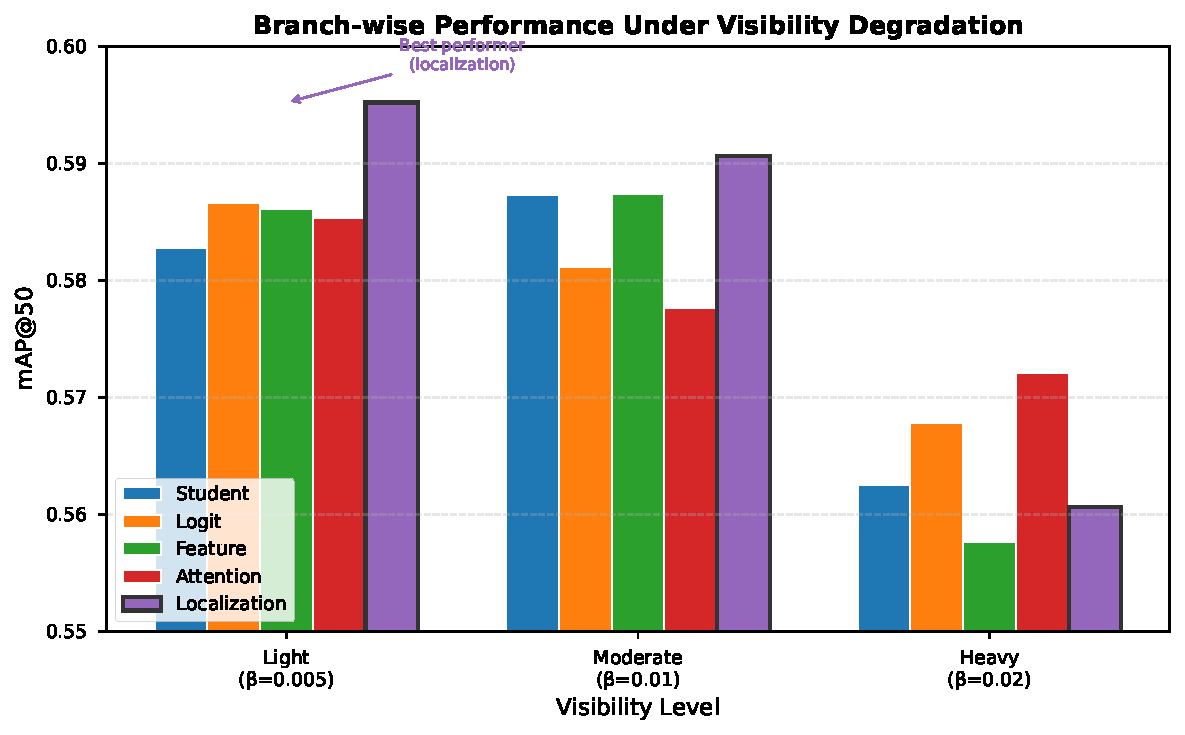
\includegraphics[width=0.85\columnwidth]{figures/figure2_branch_performance.pdf}
\caption{可见度退化下的分支级性能。定位蒸馏在轻度和中度可见度下达到最高性能，而所有分支在重度退化下收敛。}
\label{fig:branch_performance}
\end{figure}

\subsection{KD增益分析}

为量化各分支的相对有效性，\cref{tab:gain_matrix}呈现相对于仅学生基线计算的KD增益。

\begin{table}[htbp]
\centering
\caption{KD增益矩阵（相对于仅学生基线的mAP@50提升）。正值表示有益转移；负值表示负转移。}
\label{tab:gain_matrix}
\begin{tabular}{@{}lccc@{}}
\toprule
KD分支 & 轻度 & 中度 & 重度 \\
\midrule
仅logit & +0.0038 & $-$0.0062 & +0.0053 \\
仅特征 & +0.0033 & +0.0001 & $-$0.0049 \\
仅注意力 & +0.0025 & $-$0.0096 & +0.0096 \\
\textbf{仅定位} & \textbf{+0.0124} & \textbf{+0.0033} & $-$0.0019 \\
\bottomrule
\end{tabular}
\end{table}

\textbf{发现4：定位蒸馏在轻-中度退化下提供一致增益。}在轻度（+1.24\%）和中度（+0.33\%）下，定位蒸馏是唯一在重度退化前持续超越基线的分支。

\textbf{发现5：负转移发生。}特征蒸馏在重度可见度损失下表现出负转移（$-0.49\%$），提示直接特征对齐可能传播损害学生泛化的域特定偏差。

\textbf{发现6：重度退化消除KD收益。}在$\beta=0.02$下，没有分支保持对仅学生基线的明显正增益。这表明一个根本限制：当可见度损失变得严重时，教师知识本身退化，没有蒸馏机制能完全补偿。

\Cref{fig:gain_analysis}可视化相对于仅学生基线的KD增益。

\begin{figure}[htbp]
\centering
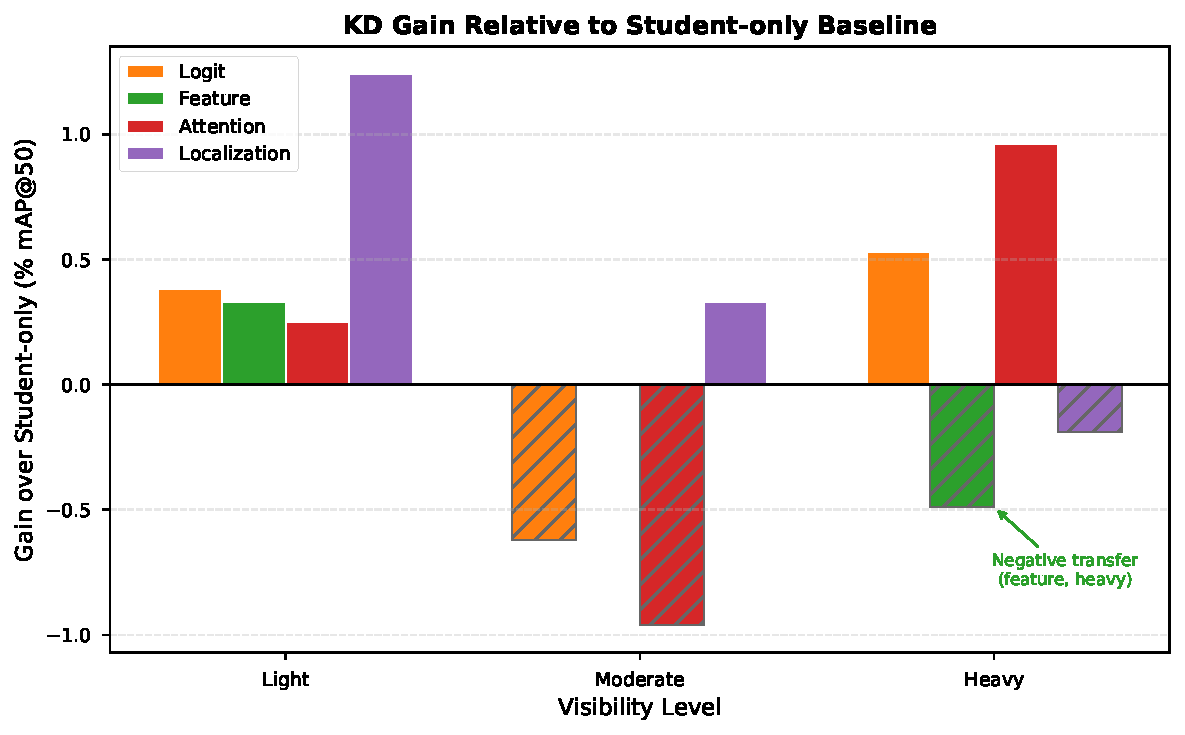
\includegraphics[width=0.85\columnwidth]{figures/figure3_gains.pdf}
\caption{相对于仅学生基线的KD增益。正值（虚线上方）表示有益转移；负值表示负转移。带斜线的柱表示负转移。}
\label{fig:gain_analysis}
\end{figure}

\subsection{排序稳定性分析}

为评估分支级结构是否跨可见度条件持续，我们计算可见度等级间的Kendall $\tau$排序相关。\Cref{tab:rankings}展示每个可见度等级下的分支排序。

\begin{table}[htbp]
\centering
\caption{每个可见度等级下按mAP@50的分支排序。排序1为最佳。}
\label{tab:rankings}
\begin{tabular}{@{}lccccc@{}}
\toprule
可见度 & 排序1 & 排序2 & 排序3 & 排序4 & 排序5 \\
\midrule
轻度 & 定位 & logit & 特征 & 注意力 & 学生 \\
中度 & 定位 & 特征 & 学生 & logit & 注意力 \\
重度 & 注意力 & logit & 学生 & 定位 & 特征 \\
\bottomrule
\end{tabular}
\end{table}

排序间的Kendall $\tau$相关：
\begin{itemize}
    \item 轻度 vs. 中度：$\tau = 0.40$，$p = 0.48$
    \item 中度 vs. 重度：$\tau = -0.80$，$p = 0.08$
    \item 轻度 vs. 重度：$\tau = -0.20$，$p = 0.82$
\end{itemize}

\textbf{发现7：部分排序稳定性，重度退化为异常值。}轻度-中度比较显示适度正相关，提示分支级结构在轻度可见度损失下部分持续。然而，重度退化产生根本不同的排序（相对于中度$\tau = -0.80$），表明控制KD有效性的机制在严重遮挡下发生质性变化。

\subsection{Phase 1：遮挡控制实验}

为进一步检验M2（遮挡）假设，我们设计了一个补充性的控制实验，直接操控遮挡率（occlusion ratio），而非通过大气散射间接改变可见度。该实验的目的不是取代前述雾天主实验，而是为后续机制分析提供额外的、干预式证据。\Cref{tab:phase1_summary}给出其中最关键的结果切片。

\begin{table}[htbp]
\centering
\caption{Phase 1遮挡控制实验摘要（mAP@50）。}
\label{tab:phase1_summary}
\begin{tabular}{@{}lccc@{}}
\toprule
遮挡率 & 学生基线 & Logit蒸馏 & 定位蒸馏 \\
\midrule
0.0（无遮挡）
& 0.4569
& 0.4071\dag
& \textbf{0.4792} (+4.9\%) \\
0.2（中度）
& 0.4693
& \textbf{0.4708}
& 0.4666 \\
0.4（重度）
& \textbf{0.4792}
& \textbf{0.4792}
& 0.4700 \\
\bottomrule
\end{tabular}
\vspace{5pt}
\small
\dag\ 训练异常。括号内为相对于学生基线的增益。
\end{table}

\textbf{Phase 1补充观察：}
\begin{enumerate}
    \item 在无遮挡条件下，localization蒸馏相对student基线具有更明显优势，而这一优势在较高遮挡率下减弱。
    \item 随着遮挡率升高，不同KD方法之间的性能差距缩小，说明遮挡会削弱KD分支间的差异。
    \item student基线在高遮挡率下未继续落后于KD方法，这提示遮挡可能改变了蒸馏收益的相对结构，但这一现象更适合被视为辅助观察，而非全文主结论。
\end{enumerate}

总体上，Phase 1与雾天主实验在方向上是一致的：当空间可见信息被进一步遮挡时，定位分支的相对优势不再稳定。这一结果为\cref{sec:mechanism}中关于M2的讨论提供了补充证据，但本文的主结论仍主要建立在雾天主实验与机制相关分析之上。

\subsection{观测总结}

我们的结构化观测阶段首先由雾天主实验建立分支级结构，而Phase 1控制实验则提供了针对遮挡作用的补充性支持。综合来看，我们得到：
\begin{enumerate}
    \item 分支级性能结构确实存在且具有统计意义；
    \item Logit蒸馏尽管广泛使用，对可见度退化检测并非最优；
    \item 定位蒸馏在轻-中度退化下表现出相对鲁棒性，但高退化时优势消失；
    \item 重度可见度损失代表所有KD机制趋于收敛的关键区域；
    \item 补充性的遮挡控制实验进一步提示：遮挡很可能是导致上述变化的重要因素之一。
\end{enumerate}

这些观测促使\cref{sec:mechanism}的机制分析，我们在其中测试特定假设以解释这些模式为何出现。
